\subsection{Calibration}
\frame{\tableofcontents[currentsubsection]}

\begin{frame}{Main Task: Find Critical Threshold with Level $\alpha$ at $\theta_0$}
\begin{figure}
    \centering
    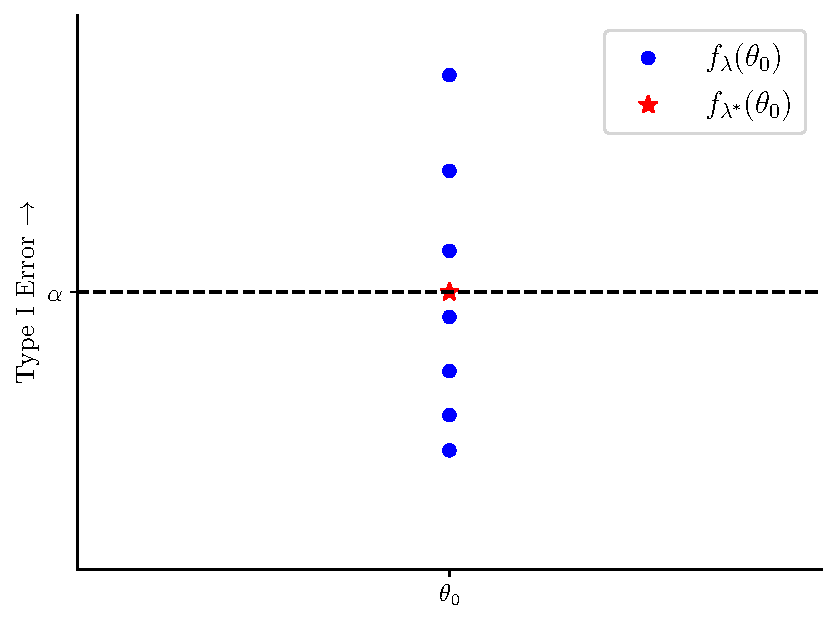
\includegraphics[width=0.95\linewidth]{figs/calibration_point_null.pdf}
\end{figure} 
\end{frame}

\begin{frame}{Straightforward for a Single Point}
\begin{itemize}
    \item Let $S(X)$ be the test statistic with data $X$.
    \item Design $\design$: rejects if $S(X) < \lambda$.
    \item Given $S_1,\ldots, S_N$ i.i.d. test statistics,
        \begin{align*}
            \hat{\lambda}^* := S_{\floor{(N+1) \alpha}}
            \implies
            \EEE\br{f_{\hat{\lambda}^*}(\theta_0)} \leq \alpha
        \end{align*}
    \item Easy to show using Beta distribution.
\end{itemize} 
\end{frame}

\begin{frame}{Calibration Results for a Single Point}
\begin{figure}
    \centering
    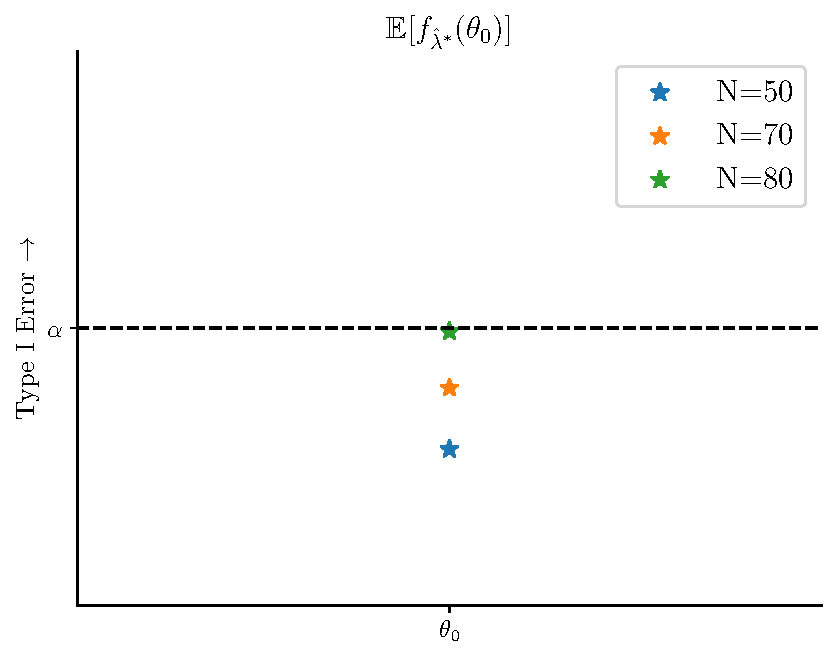
\includegraphics[width=0.9\linewidth]{figs/calibration_point_null_solution.pdf}
\end{figure} 
\end{frame}

\begin{frame}{Main Task: Find Critical Threshold with Level $\alpha$ at $\theta$}
 \begin{figure}
     \centering
     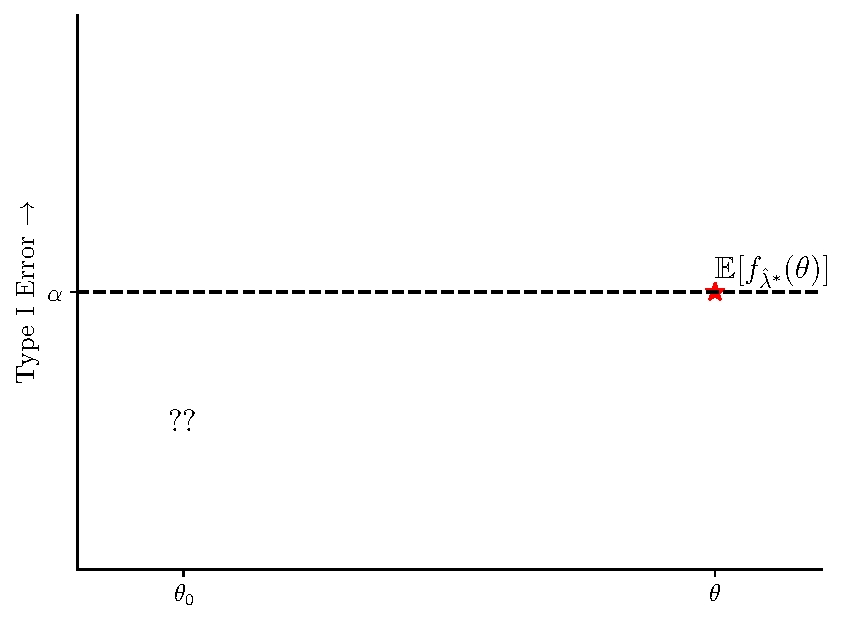
\includegraphics[width=0.95\linewidth]{figs/calibration_tile.pdf}
 \end{figure}
\end{frame}

\begin{frame}{Inverted Tilt-Bound}
Claim: Calibrate at $\theta_0$ to Control Tilt-Bound at $\theta$
\begin{figure}
    \centering
    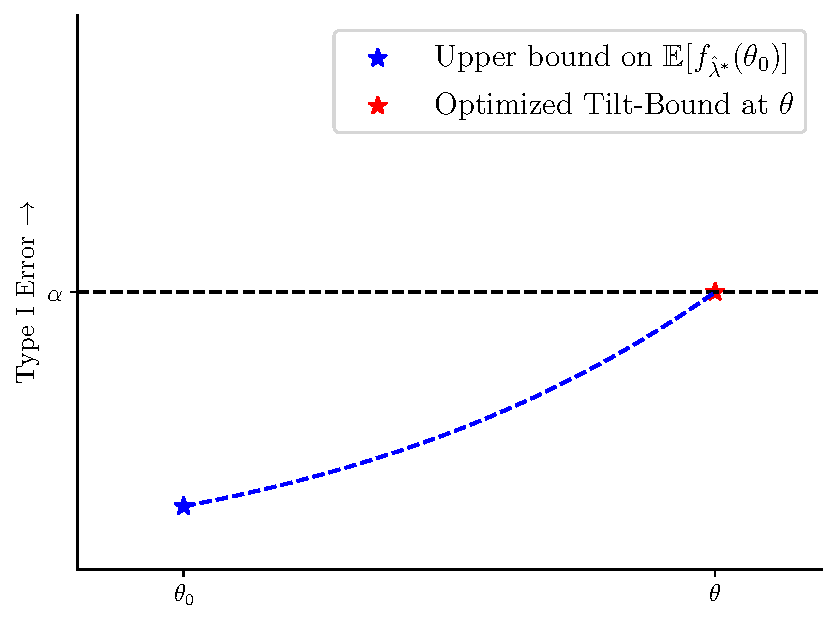
\includegraphics[width=0.9\linewidth]{figs/calibration_tile_solution.pdf}
\end{figure} 
\end{frame}

%\begin{frame}{Extending point-null case to a tile using CSE}
%\begin{itemize}
%    \item Assume $\Theta$ a region around a point $\theta_0$.
%    \item Back-solve from the worst-case Tilt-bound over $\Theta$ (which always occurs at a corner of $\Theta$).
%    \item Find a level $\alpha' < \alpha$ so that
%    \begin{equation}
%        \EEE\br{f_{\lambda}(\theta_0)} \leq \alpha' 
%        \implies
%        \sup \limits_{\theta \in \Theta}
%        \EEE\br{f_{\lambda}(\theta)} \leq \alpha
%    \end{equation}
%    \item Then it suffices to point-calibrate at $\theta_0$ with target level $\alpha'$.
%\end{itemize} 
%\end{frame}

\begin{frame}{Use CSE to Control Type I Error at $\theta$}
\begin{align*}
    \EEE\br{f_{\lambda}(\theta_0+v)}
    &\leq
    U(\theta_0, v, q, \EEE\br{f_{\lambda}(\theta_0)})
\end{align*} 
\begin{itemize}
    \item Back-solve to hit level $\alpha$:
        \begin{align*}
            U(\theta_0, v, q, \EEE\br{f_{\lambda}(\theta_0)})
            \leq 
            \alpha
            \iff
            \EEE\br{f_\lambda(\theta_0)}
            \leq 
            U^{-1}(\theta_0, v, q, \alpha)
        \end{align*}
\end{itemize} 
\textbf{Inverted Tilt-Bound:}
\begin{equation*}
    U^{-1}(\theta_0, v, q, \alpha) 
    := \pr{
    \alpha \exp\br{
    -\frac{\psi(\theta_0, v, q)}{q} 
    + \psi(\theta_0, v, 1)
    }}^{\frac{q}{q-1}}
\end{equation*}
\end{frame}

\begin{frame}{Use Point-Null Case to Find Critical Threshold}
\begin{itemize}
    \item Let $\alpha' := U^{-1}(\theta_0, v, q, \alpha)$.
    \item Find $\hat{\lambda}^*$ such that
        \begin{align*}
            \EEE\br{f_{\hat{\lambda}^*}(\theta_0)} \leq \alpha'
        \end{align*}
    \item Maximize $\alpha'$ over $q \geq 1$ 
        for free to get least-conservative threshold.
\end{itemize} 
Then,
\begin{align*}
    \EEE\br{f_{\hat{\lambda}^*}(\theta_0 + v)}
    \leq
    U(\theta_0, v, q, \EEE\br{f_{\hat{\lambda}^*}(\theta_0)})
    \leq
    \alpha
\end{align*}
\end{frame}

\begin{frame}{Control Type I Error in a Region}
\begin{itemize}
    \item Back-solve with \textbf{worst-case} Tilt-Bound:
        \begin{align*}
            &\sup\limits_{v \in \Theta-\theta_0}
            U(\theta_0, v, q, \EEE\br{f_{\lambda}(\theta_0)})
            \leq 
            \alpha
            \\\iff \quad
            &\EEE\br{f_\lambda(\theta_0)}
            \leq 
            \inf\limits_{v \in \Theta-\theta_0}
            U^{-1}(\theta_0, v, q, \alpha)
        \end{align*}
    \item Let $\alpha' := \inf\limits_{v \in \Theta -\theta_0} U^{-1}(\theta_0, v, q, \alpha)$.
    \item Maximize $\alpha'$ over $q \geq 1$.
    \item Find $\hat{\lambda}^*$ such that 
        \begin{align*}
            \EEE\br{f_{\hat{\lambda}^*}(\theta_0)} \leq \alpha'
        \end{align*}
\end{itemize} 
\end{frame}

\begin{frame}{How to optimize over $v$?}
\begin{align*}
    \inf\limits_{v \in \Theta-\theta_0}
    U^{-1}(\theta_0, v, q, \alpha)
\end{align*} 
\begin{itemize}
    \item \textbf{Assume a linearity condition}!
    \item Inverted Tilt-Bound is \textbf{quasi-concave} in $v$, respectively!
    \item If $\Theta$ is a polytope, suffices to compute only at the vertices!
\end{itemize} 
\end{frame}

\begin{frame}{How to optimize over $v$?}
\begin{theorem}[Quasi-convex in $v$]
Let $\set{P_{\theta} : \theta \in \Theta \subseteq \R^d}$ be a family of distributions:
\begin{align*}
    dP_{\theta}(x) = \exp\sbr{g_{\theta}(x) - A(\theta)} d\mu(x)
\end{align*}
Fix any $\theta_0 \in \Theta$.
Suppose that $\Delta(v, x) \equiv g_{\theta_0+v}(x) - g_{\theta_0}(x)$ 
is linear in $v$, i.e.
$\Delta(v, x) = W(x)^\top v$ 
for some $W(x) \in \R^d$.
Then, the Inverted Tilt-Bound is quasi-concave as a function of $v$.
\end{theorem}
\end{frame}

\begin{frame}{Divide-and-Conquer yields a Global Guarantee}
\begin{itemize}
    \item Assume $\Theta$ any bounded space.
    \item Partition $\Theta$ into tiles $\set{\Theta_i}_{i=1}^I$ 
        with representatives $\set{\theta_i}_{i=1}^I$.
    \item Calibrate to get $\hat{\lambda}^*_i$ for each tile $\Theta_i$.
    \item Take the most conservative, $\hat{\lambda}^* := \min\limits_{i=1,\ldots, I} \hat{\lambda}^*_i$.
    \item Then,
        \begin{align*}
            \sup\limits_{\theta \in \Theta}
            \EEE\br{f_{\hat{\lambda}^*}(\theta)}
            &=
            \max\limits_{i=1,\ldots,I}
            \sup\limits_{\theta \in \Theta_i}
            \EEE\br{f_{\hat{\lambda}^*}(\theta)}
            \\&\leq 
            \max\limits_{i=1,\ldots,I}
            \sup\limits_{\theta \in \Theta_i}
            \EEE\br{f_{\hat{\lambda}^*_i}(\theta)}
            \\&\leq
            \alpha
        \end{align*}
\end{itemize} 
\end{frame}

\begin{frame}{Type I Error Tightens with More Simulations and Tiles}
\begin{figure}
    \centering
    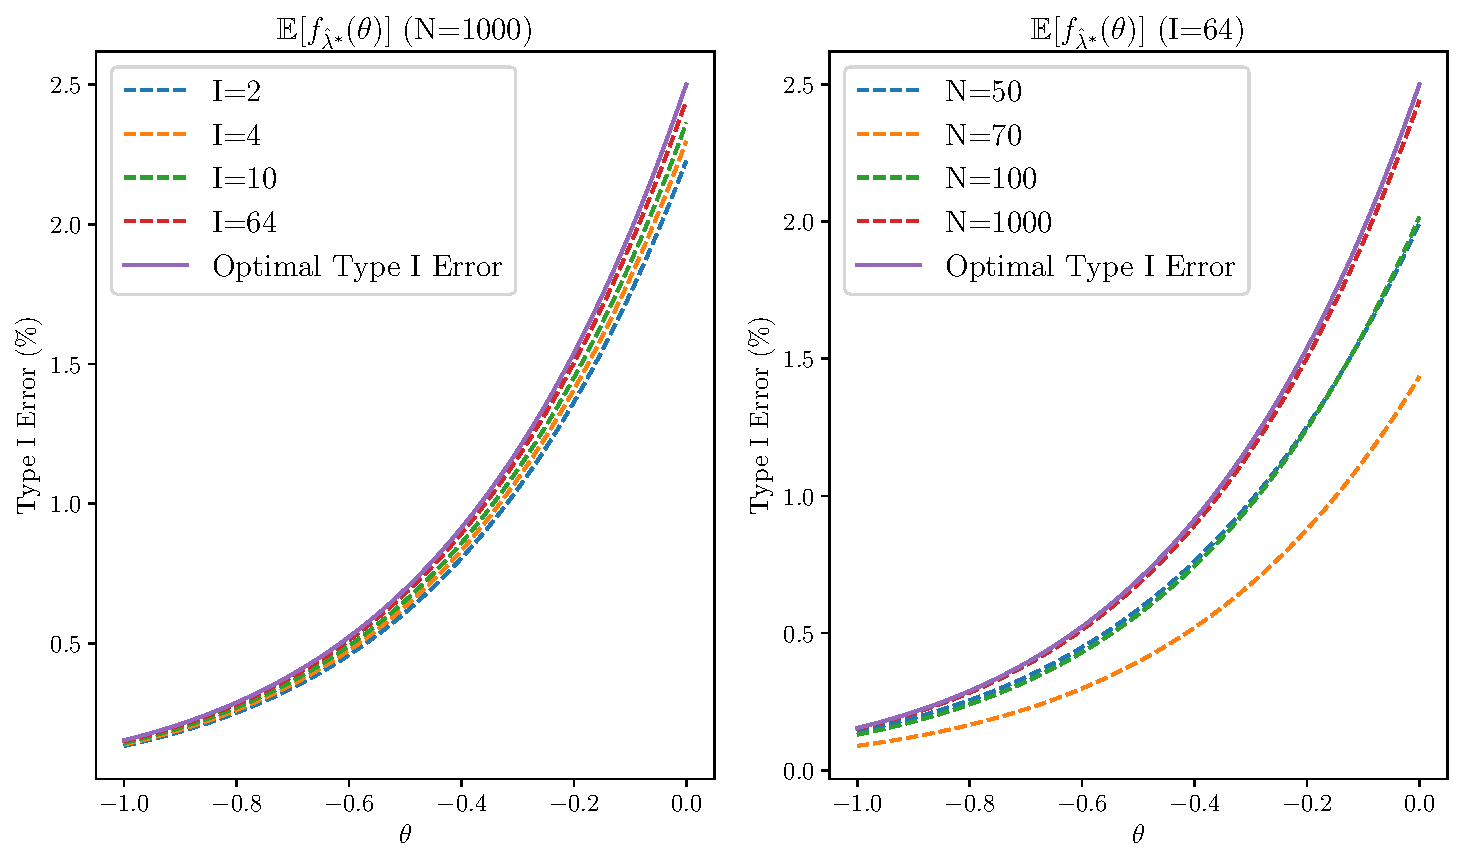
\includegraphics[width=\linewidth]{figs/calibration_z_test.pdf}
\end{figure} 
\end{frame}


